\documentclass{beamer}
% Use DS9 global theme
\usepackage{../../../../shared/templates/ds9_theme}

% Title page configuration
\title[ Vector Analysis]{PHYS11 CH:5.1-5.3}
\subtitle{Vector Analysis and Applications }
\author[Mr. Gullo]{Mr. Gullo}
\date[Oct 2024]{October 2024}

% Table of contents at the beginning of each section
\AtBeginSection[]
{
  \begin{frame}
    \frametitle{Table of Contents}
    \tableofcontents[currentsection]
  \end{frame}
}

\begin{document}

\frame{\titlepage}

\begin{frame}
\frametitle{Learning Objectives}
By the end of this lesson, you will be able to:
\pause
\begin{itemize}
    \item Understand and apply graphical methods for vector addition \pause
    \item Use the tip-to-tail method to add vectors graphically \pause
    \item Apply analytical methods to add and subtract vectors \pause
    \item Resolve vectors into perpendicular components \pause
    \item Calculate magnitude and direction of resultant vectors \pause
    \item Solve real-world physics problems using vector analysis
\end{itemize}
\end{frame}

\section{Graphical Methods for Vector Addition}

\begin{frame}
\frametitle{What is a Vector?}
\begin{itemize}
    \item A \textbf{vector} is a quantity that has both magnitude and direction \pause
    \item Examples: displacement, velocity, acceleration, force \pause
    \item A \textbf{scalar} has only magnitude \pause
    \item Examples: distance, speed, mass, temperature \pause
\end{itemize}
\vspace{0.3cm}
\textbf{Vector Notation:} $\vec{A}$ or $\mathbf{A}$
\end{frame}

\begin{frame}
\frametitle{Trigonometry Review}
\begin{columns}[T] % Top-aligned columns
    \column{0.48\textwidth}
    \begin{figure}
        \centering
        \includegraphics[width=\linewidth]{phys11-math-trigonometry-sohcahtoa.png}
        \caption{SOHCAHTOA mnemonic}
    \end{figure}

    \column{0.48\textwidth}
    \begin{figure}
        \centering
        \includegraphics[width=\linewidth]{phys11-math-sine-cosine-laws.png}
        \caption{Sine and Cosine Laws}
    \end{figure}
\end{columns}
\end{frame}

\begin{frame}
\frametitle{Graphical Vector Addition: Tip-to-Tail Method}
\textbf{Steps:}
\pause
\begin{enumerate}
    \item Draw the first vector to scale with proper direction \pause
    \item Place the tail of the second vector at the tip of the first \pause
    \item Draw the resultant from the tail of the first to the tip of the last \pause
    \item Measure the magnitude and direction of the resultant
\end{enumerate}
\pause
\vspace{0.3cm}
\textbf{Important:} Vector addition is commutative: $\vec{A} + \vec{B} = \vec{B} + \vec{A}$

\vspace{0.2cm}
\alert{[See Figure 5.3 - Tip-to-tail method illustration]}
\end{frame}

\section{Analytical Methods for Vector Addition}

\begin{frame}
\frametitle{Vector Addition and Subtraction}
\begin{itemize}
    \item Vector addition:
- Tip-to-tail method
- Parallelogram method

\item Vector subtraction:
- Add the negative of the vector: $\vec{A} - \vec{B} = \vec{A} + (-\vec{B})$

\item Resultant vector: $\vec{R} = \vec{A} + \vec{B}$
 \\
- For n vectors: $\vec{R} = \vec{A} + \vec{B} + \vec{C} + ... + \vec{N}$
\end{itemize}
\end{frame}

\begin{frame}
\frametitle{Vector Addition and Subtraction}
\begin{itemize}
\item Magnitude of resultant:\\
- General case: $|\vec{R}| = \sqrt{A^2 + B^2 + 2AB\cos\theta}$\\
- For perpendicular vectors: $|\vec{R}| = \sqrt{A^2 + B^2}$

\item Direction of resultant:\\
- Using magnitudes and angle: $\tan\phi = \frac{B\sin\theta}{A + B\cos\theta}$\\
- Using components: $\tan\phi = \frac{A_y + B_y}{A_x + B_x}$, 

\end{itemize}
\end{frame}

\begin{frame}
\frametitle{Resolving Vectors into Components}
\begin{itemize}
    \item Any vector can be resolved into x and y components
    \item $A_x = A\cos\theta$, $A_y = A\sin\theta$
    \item Magnitude: $A = \sqrt{A_x^2 + A_y^2}$
    \item Direction: $\tan\theta = \frac{A_y}{A_x}$
\end{itemize}

\vspace{0.3cm}
\alert{[See Figure 5.7 - Vector components diagram]}
\end{frame}

\section{Vector Applications and Problem Solving}

\begin{frame}
\frametitle{Example 1: River Crossing Problem - Setup}
\textbf{Problem:} A river flows SW to NE at 7.1 m/s. A boat moving at 13 m/s wants to reach a point due east. At what angle should the boat head?
\pause
\vspace{0.3cm}

\begin{columns}[T]
\column{0.48\textwidth}
\textbf{G - Givens}
\begin{itemize}
\item $v_r = 7.1$ m/s (SW to NE)
\item $v_b = 13$ m/s
\item Direction: due east
\end{itemize}

\column{0.48\textwidth}
\textbf{U - Unknown}
\begin{itemize}
\item Angle $\theta = ?$
\item (relative to east)
\end{itemize}
\end{columns}
\end{frame}

\begin{frame}
\frametitle{Example 1: River Crossing Problem - Equation}
\textbf{E - Equation}
\begin{itemize}
\item River components: $v_{rx} = v_r\cos 45°$, $v_{ry} = v_r\sin 45°$ \pause
\item For eastward motion: $v_{by} = -v_{ry}$ \pause
\item Angle: $\theta = \arcsin(v_{by}/v_b)$
\end{itemize}
\end{frame}

\begin{frame}
\frametitle{Example 1: River Crossing Problem - Solution}
\textbf{S - Substitute}
\begin{itemize}
\item $v_{rx} = v_{ry} = 7.1\cos 45° = 5.02$ m/s \pause
\item $v_{by} = -5.02$ m/s \pause
\item $\theta = \arcsin(-5.02/13)$
\end{itemize}
\pause

\textbf{S - Solve}
\begin{itemize}
\item $\theta \approx -22.6°$
\item \boxed{\text{The boat should head } 22.6° \text{ south of east}}
\end{itemize}
\end{frame}

\begin{frame}
\frametitle{Example 2: Displacement Problem - Setup}
\textbf{Problem:} A person walks 10.0 m north, then 2.0 m east. Find the resultant displacement.
\pause
\vspace{0.3cm}

\begin{columns}[T]
\column{0.48\textwidth}
\textbf{G - Givens}
\begin{itemize}
\item $d_1 = 10.0$ m (north)
\item $d_2 = 2.0$ m (east)
\end{itemize}

\column{0.48\textwidth}
\textbf{U - Unknown}
\begin{itemize}
\item Magnitude: $R = ?$
\item Direction: $\theta = ?$
\end{itemize}
\end{columns}
\end{frame}

\begin{frame}
\frametitle{Example 2: Displacement Problem - Equation}
\textbf{E - Equation}
\begin{itemize}
\item Pythagorean theorem: $R = \sqrt{d_1^2 + d_2^2}$ \pause
\item Direction: $\theta = \arctan(d_1/d_2)$
\end{itemize}
\end{frame}

\begin{frame}
\frametitle{Example 2: Displacement Problem - Solution}
\textbf{S - Substitute and Solve}
\begin{itemize}
\item $R = \sqrt{(10.0)^2 + (2.0)^2}$ \pause
\item $R = \sqrt{100 + 4} = \sqrt{104} \approx 10.2$ m \pause
\item $\theta = \arctan(10.0/2.0) = \arctan(5.0) \approx 78.7°$
\end{itemize}
\pause

\textbf{Answer:}
\begin{itemize}
\item \boxed{\vec{R} = 10.2 \text{ m, } 78.7° \text{ north of east}}
\end{itemize}
\end{frame}
\section{Projectile Motion (Section 5.3)}

\begin{frame}
\frametitle{What is Projectile Motion?}
\begin{itemize}
    \item An object moving through the air under the influence of gravity only \pause
    \item Examples: thrown ball, kicked soccer ball, fired cannon \pause
    \item Two independent motions:
    \begin{itemize}
        \item Horizontal: constant velocity (no acceleration) \pause
        \item Vertical: constant acceleration ($a = -g = -9.8$ m/s²)
    \end{itemize}
\end{itemize}
\pause
\vspace{0.3cm}
\textbf{Key Assumption:} Air resistance is negligible

\vspace{0.2cm}
\alert{[See Figure 5.27 - Projectile motion trajectory]}
\end{frame}

\begin{frame}
\frametitle{Projectile Motion Equations}
\textbf{Horizontal Motion:}
\begin{itemize}
    \item $v_x = v_0 \cos\theta$ (constant) \pause
    \item $x = v_0 t \cos\theta$ \pause
\end{itemize}

\textbf{Vertical Motion:}
\begin{itemize}
    \item $v_y = v_0 \sin\theta - gt$ \pause
    \item $y = v_0 t \sin\theta - \frac{1}{2}gt^2$ \pause
\end{itemize}

\textbf{Special Formulas:}
\begin{itemize}
    \item Range: $R = \frac{v_0^2 \sin(2\theta)}{g}$ \pause
    \item Maximum height: $h_{\max} = \frac{v_0^2 \sin^2\theta}{2g}$
\end{itemize}

\vspace{0.2cm}
\alert{[See Figure 5.29 - Horizontal and vertical components of projectile motion]}
\end{frame}

\begin{frame}
\frametitle{Example 3: Projectile Motion - Setup}
\textbf{Problem:} A water-balloon cannon fires at 30 m/s, 50° above horizontal. Find the range.
\pause
\vspace{0.3cm}

\begin{columns}[T]
\column{0.48\textwidth}
\textbf{G - Givens}
\begin{itemize}
\item $v_0 = 30$ m/s
\item $\theta = 50°$
\item $g = 9.8$ m/s²
\end{itemize}

\column{0.48\textwidth}
\textbf{U - Unknown}
\begin{itemize}
\item Range: $R = ?$
\end{itemize}
\end{columns}
\end{frame}

\begin{frame}
\frametitle{Example 3: Projectile Motion - Equation}
\textbf{E - Equation}
\begin{itemize}
\item Range formula: $R = \frac{v_0^2 \sin(2\theta)}{g}$ \pause
\item Note: $\sin(2\theta) = \sin(2 \times 50°) = \sin(100°)$
\end{itemize}
\end{frame}

\begin{frame}
\frametitle{Example 3: Projectile Motion - Solution}
\textbf{S - Substitute}
\begin{itemize}
\item $R = \frac{(30)^2 \sin(100°)}{9.8}$ \pause
\item $R = \frac{900 \times 0.9848}{9.8}$ \pause
\item $R = \frac{886.3}{9.8}$
\end{itemize}
\pause

\textbf{S - Solve}
\begin{itemize}
\item $R \approx 90.4$ m
\item \boxed{\text{The water balloon will fall approximately } 90.4 \text{ m away}}
\end{itemize}
\end{frame}
\begin{frame}
\frametitle{Reading Homework}
\textbf{Additional Topics for Self-Study:}
\pause
\begin{itemize}
    \item \textbf{Section 5.4:} Inclined Planes \pause
    \begin{itemize}
        \item Forces on inclined surfaces
        \item Normal and parallel components
        \item Friction on slopes
    \end{itemize}
    \pause
    \item \textbf{Section 5.5:} Simple Harmonic Motion \pause
    \begin{itemize}
        \item Oscillatory motion
        \item Springs and pendulums
        \item Period and frequency
    \end{itemize}
\end{itemize}
\pause
\vspace{0.3cm}
\textbf{Note:} These sections will be covered in future lessons
\end{frame}

\begin{frame}
\frametitle{Summary: Sections 5.1-5.3}
\textbf{Section 5.1 - Graphical Methods:}
\begin{itemize}
    \item Tip-to-tail method for vector addition
\end{itemize}
\pause

\textbf{Section 5.2 - Analytical Methods:}
\begin{itemize}
    \item Resolving vectors into components
    \item Using trigonometry for vector calculations
\end{itemize}
\pause

\textbf{Section 5.3 - Projectile Motion:}
\begin{itemize}
    \item Independent horizontal and vertical motion
    \item Key equations for range, height, and time
\end{itemize}
\pause

\vspace{0.3cm}
\textbf{Practice problems are essential for mastery!}
\end{frame}

\begin{frame}
\frametitle{Global Angles}

\begin{block}{Problem}
What is the global angle of 20° south of west?
\end{block}

\begin{center}
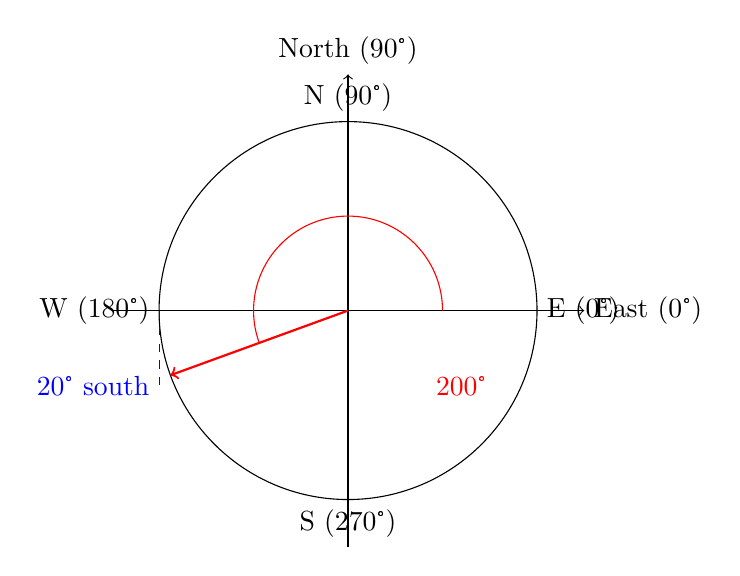
\begin{tikzpicture}[scale=1.2]
    % Draw main circle
    \draw (0,0) circle (2);
    
    % Draw axes
    \draw[->] (-2.5,0) -- (2.5,0) node[right] {East (0°)};
    \draw[->] (0,-2.5) -- (0,2.5) node[above] {North (90°)};
    
    % Draw compass directions
    \node[above] at (0,2) {N (90°)};
    \node[left] at (-2,0) {W (180°)};
    \node[right] at (2,0) {E (0°)};
    \node[below] at (0,-2) {S (270°)};
    
    % Draw the angle
    \draw[->, thick, red] (0,0) -- ({2*cos(200)}, {2*sin(200)});
    \draw[red] (1,0) arc (0:200:1);
    
    % Label the angle
    \node[red] at (1.2,-0.8) {200°};
    
    % Show the "south of west" reference
    \draw[blue, dashed] (-2,0) -- (-2,-0.8) node[left] {20° south};
    
\end{tikzpicture}
\end{center}
\end{frame}

\begin{frame}
\frametitle{River Crossing Problem}
\begin{block}{Problem}
A person attempts to cross a river in a straight line by navigating a boat at $15 \mathrm{~m} / \mathrm{s}$. If the river flows at $5.0 \mathrm{~m} / \mathrm{s}$ from left to right, what would be:
\begin{itemize}
    \item The magnitude of the boat's resultant velocity?
    \item The direction relative to the straight line across the river?
\end{itemize}
\end{block}

\begin{center}
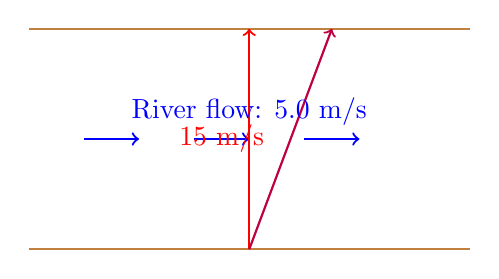
\begin{tikzpicture}[scale=0.7]
    % River banks
    \draw[thick, brown] (-4,2) -- (4,2);
    \draw[thick, brown] (-4,-2) -- (4,-2);
    
    % River flow arrows
    \draw[->, blue, thick] (-3,0) -- (-2,0);
    \draw[->, blue, thick] (-1,0) -- (0,0);
    \draw[->, blue, thick] (1,0) -- (2,0);
    
    % Boat's intended direction
    \draw[->, thick, red] (0,-2) -- (0,2);
    
    % Resultant motion
    \draw[->, thick, purple] (0,-2) -- (1.5,2);
    
    % Labels
    \node[blue] at (0,0.5) {River flow: $5.0 \mathrm{~m}/\mathrm{s}$};
    \node[red] at (-0.5,0) {$15 \mathrm{~m}/\mathrm{s}$};
\end{tikzpicture}
\end{center}

\end{frame}

\begin{frame}
\frametitle{River Crossing Solution}

The correct solution:
\begin{itemize}
    \item Resultant velocity: $15.8 \mathrm{~m} / \mathrm{s}$
    \item Direction: $18.4^{\circ}$ to the right
\end{itemize}


Using the Pythagorean theorem:
\[v_\text{resultant} = \sqrt{(5.0)^2 + (15.0)^2} = 15.8 \mathrm{~m}/\mathrm{s}\]

The angle is given by:
\[\theta = \tan^{-1}\left(\frac{5.0}{15.0}\right) = 18.4^\circ\]

\end{frame}

\end{document}